\documentclass[10pt]{beamer}

%Language package english
\usepackage[english]{babel}
\usepackage[T1]{fontenc}
\usepackage[utf8]{inputenc}

\usepackage{dutchcal}        %nice Hilbertspace symbols
\usepackage{braket}          %for braket notation

%\setbeamercovered{transparent}  %in order to see shape of the following bullet points 

%for striking out text
\usepackage[normalem]{ulem}




%fuer Identitaet 
\usepackage{dsfont}


%Aussehen der Präsentation
\usetheme{Boadilla}
\usecolortheme{sidebartab}

%\usepackage{lmodern}		% nice schriftart
%\usepackage{etoolbox}        %reformat sections etc.
%---------------------------- definitions
%\newcommand{\el}{ {\scriptstyle{\in}}\; }


\newcommand{\Hilb}{ {\mathcal{H}} }
\newcommand{\dualHilb}{ {\mathcal{H}^*} }
\newcommand{\Haml}{ {\hat{H}} }
\newcommand{\modul}[1]{{\left|{#1}\right|}}
\newcommand{\norm}[1]{\ensuremath{ \Vert {#1} \Vert}}
\newcommand{\trace}[1]{\ensuremath{\text{Tr} \, {#1} }}
\newcommand{\QC}{\ensuremath{\textup{QC}}}
\newcommand{\LC}{\ensuremath{\textup{LC}}}
\newcommand{\sclr}[2]{\ensuremath{\langle{#1},{#2}\rangle}}
\newcommand{\tensor}{\ensuremath{\otimes}}


\DeclareMathOperator*{\esssup}{ess\,sup} % essentiellen Supremums
\DeclareMathOperator{\spn}{span} % Span
\DeclareMathOperator{\supp}{supp} % Träger
\DeclareMathOperator{\proj}{proj} % Träger
\DeclareMathOperator{\tr}{Tr} 
\DeclareMathOperator{\sgn}{sign}
 %----- put in Preamble
\begin{document}

		\author{Maxi Brandstetter, Felix Kirschner, Arne Heimendahl}
		\title{Ungleichungen und ähnlich verwirrende Konzepte}
		\subtitle{Coffee}
		\institute[]{University of Cologne}
			\date{\today}
		\begin{frame}
		\maketitle
	\end{frame}
	
%	\section{Introduction}
\subsection{ksjladüys}
\begin{frame}{Outline}
\tableofcontents[currentsection]
\end{frame}


\begin{frame}{Let's get on the same page}
 \begin{itemize}
  \item \large{We should know what a \textit{state} is}
  \item \large{We should know what the \textit{tensor product} does}
  \item \large{We should be familiar with the \textit{Dirac notation}}
 \end{itemize}
\end{frame}

\begin{frame}{Quantum systems}
\begin{itemize}
\item A quantum system is a portion of the whole universe. For example a set electrons. 
\item A quantum system $X$ is associated with a copy of $\mathbb{C}^k$ 
\item It may consist of subsystems $X_1, \dots , X_N$ each of which is associated with a copy of $\mathbb{C}^{n_i}$. In this case $k = n_1 \dots n_N$
\end{itemize}
\end{frame}

\begin{frame}{Measurements}
\begin{itemize}
    \item A measurement can be performed on a system $X$ that is in state $\rho$
    \item Let $\mathcal{A}$ be a finite set of outcomes of the measurement
    \item The measurement itself is defined by a set of psd matrices $\{ F^a \}_{a\in \mathcal{A}} \subseteq \mathbb{C}^{n \times n}$ that sum up to the identity matrix, i.e. $\sum_{a \in \mathcal{A}} F^a = I$
\end{itemize}
\end{frame}

\begin{frame}{Measurements}
\begin{itemize}
    \item A projective measurement is defined by psd matrices that satisfy $F^aF^b = \delta_{ab}F^a \text{ } \forall a,b \in \mathcal{A}$
    \item The outcome of a measurement is a random variable $\chi$ with probability distribution: $\mathbb{P}[ \chi = a ] = \text{Tr}(\rho F^a)$
    \item To define an expected value we define outcomes in $\mathcal{A}$ as real numbers
\end{itemize}
    
\end{frame}


\begin{frame}{Measurements}
\begin{itemize}
    \item $\mathbb{E} [\chi ] = \sum_{a \in \mathcal{A}} a \text{Tr} ( \rho F^a ) =  \text{Tr} ( \rho ( \sum_{a \in \mathcal{A}} a F^a))$
    \item $\sum_{a \in \mathcal{A}} aF^a$ is called observable
    \item A simple case we will use later are $\{ -1, 1 \}$-valued observables
    \item if we consider projective measurements we have
\end{itemize}
    \begin{equation*}
(F^+-F^-)^2 = \underbrace{F^{+^2}}_{= F^+}- \underbrace{F^+F^-}_{\delta_{+-}=0} + \underbrace{F^{-^2}}_{F^-} = F^+ + F^- = I
\end{equation*}
\begin{itemize}
    \item i.e. a $\{ -1, 1 \}$-valued observable is both unitary an Hermitian 
\end{itemize}

\end{frame}

\begin{frame}{Doling out subsystems}
\begin{itemize}
    \item Consider a system $X$ consisting of subsystems $X_1, \dots X_N$ which we distribute among $N$ parties, which may be located anywhere in the universe
    \item The parties \textit{share} the state $X$ is in
    \item Every party may perform a measurement on their subsystem $X_i$, i.e. there are $N$ sets of psd matrices $\{F^{a_1} \}_{a_1 \in \mathcal{A}_1} \in \mathbb{C}^{n_1 \times n_1}, \dots , \{F^{a_N} \}_{a_N \in \mathcal{A}_N} \in \mathbb{C}^{n_N \times n_N} $
\end{itemize}
    
\end{frame}

\begin{frame}{}
    The joint probability distribution of the $N$ measurement outcomes $\chi_1 , \dots , \chi_N$ is 
\begin{equation*}
\mathbb{P}\left[ \chi_1 = a_1, \chi_2 = a_2, \dots , \chi_N = a_N \right] = \text{Tr}(\rho F_1^{a_1} \otimes \dots \otimes F_N^{a_N}) 
\end{equation*}
\end{frame}

\begin{frame}{Entanglement}
\begin{itemize}
    \item We will only consider pure states meaning states that they have rank $1$ and therefore can be written as $\rho = \vert \psi \rangle \langle \psi \vert$
    \item A state is called product state if it can be written as $\vert \psi \rangle = \vert \psi_1 \rangle \vert \psi_2 \rangle \dots \vert \psi_N \rangle$
    \item When a vector $\vert \psi \rangle$ is referred to as a state we mean the matrix $\vert \psi \rangle \langle \psi \vert$
    \item A state that is not a product state is called entangled
\end{itemize}
    
\end{frame}

\begin{frame}{Example}
    \begin{itemize}
        \item Let $\vert \psi \rangle = \vert \psi_A \rangle \vert \psi_B \rangle$ be a system and give $\vert \psi_A \rangle$ to Alice and $\vert \psi_B \rangle$ to Bob
        \item Let them perform measurements $\{ G^b \}_{b \in \mathcal{B}}$ and $\{F^a \}_{a \in \mathcal{A}}$ on their respective quantum systems
        \item What is the  probability of Alice getting measurement outcome $\chi_A = a$ and Bob getting $\chi_B = b$?
    \end{itemize}
\end{frame}

\begin{frame}{Example}
\begin{flalign*}
\text{Tr}(\vert \psi \rangle \langle \psi \vert F^a \otimes G^b ) & = \langle \psi \vert F^a \otimes G^b \vert \psi \rangle \\
& = (\langle \psi_A \vert \otimes \langle \psi_B \vert) (F^a \otimes G^b )(\vert \psi_A \rangle  \otimes \vert \psi_B \rangle )\\
& = ((\langle \psi_A \vert F^a)\otimes (\langle \psi_B \vert  G^b))( \vert \psi_A \rangle \otimes \vert \psi_B \rangle) \\
& = \langle \psi_A \vert F^a \vert \psi_A \rangle \otimes  \langle \psi_B \vert G^b \vert \psi_B \rangle \\
&= \langle \psi_A \vert F^a \vert \psi_A \rangle  \langle \psi_B \vert G^b \vert \psi_B \rangle
\end{flalign*}
This is equal to the product of the probabilities of Alice measuring $a$ and Bob measuring $b$, i.e. the outcome do not correlate.
\end{frame}

\begin{frame}{Nonlocal games}
    \begin{itemize}
        \item Three participants: Alice, Bob and a referee
        \item Referee doles out a question $s$ to Alice and a question $t$ to Bob
        \item Alice and Bob are assumed to be located anywhere in the universe respectively 
        \item Alice and Bob must not communicate
        \item Alice sends answer $a$ Bob sends answer $b$ back to the referee, who then decides whether both win or both lose
    \end{itemize}
\end{frame}

\begin{frame}{Nonlocal games}
    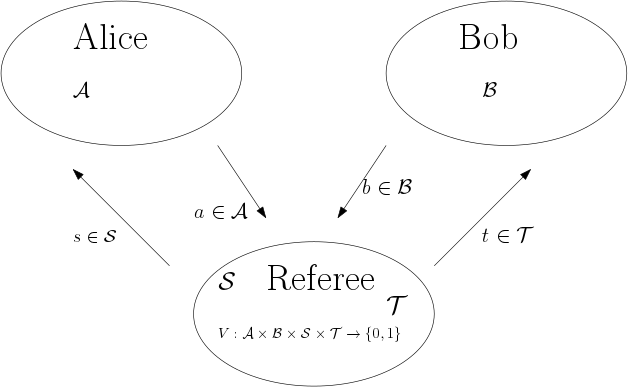
\includegraphics[scale=0.5]{Untitled.png}
\end{frame}

\begin{frame}{Mathematically speaking}
\begin{itemize}
    \item Four finite sets $\mathcal{A}, \mathcal{B}, \mathcal{S}, \mathcal{T}$
    \item probability distribution $\pi$ over $\mathcal{S} \times \mathcal{T}$ \\ $\pi : \mathcal{S} \times \mathcal{T} \rightarrow [0,1]$
    \item The referee sends with probability $\pi (s,t)$ $s$ to Alice and $t$ to Bob
    \item They answer with an element $a \in \mathcal{A}$ and $b \in \mathcal{B}$ respectively
    \item A map $V : \mathcal{S} \times \mathcal{T} \times \mathcal{A} \times \mathcal{B} \rightarrow \{ 0, 1 \}$
    \item They win if $V(s,t,a,b)=1$ and lose otherwise
\end{itemize}
\end{frame}

\begin{frame}{Classical strategies}
    \begin{itemize}
        \item All players know $\pi$ and $V$ and the information they received but not what the other players received
        \item They are allowed to agree on a strategy beforehand but must not communicate once the game started
        \item A deterministic strategy is a map $a : \mathcal{S} \rightarrow \mathcal{A}$ for Alice and $b : \mathcal{T} \rightarrow \mathcal{B}$ for Bob
        The winning probability then is:
    \end{itemize}
    \begin{equation*}
        \mathbb{E}_{s,t \sim \pi} \left[ V(a(s),b(t),s,t) \right]
\end{equation*}
\end{frame}

\begin{frame}{Quantum case}
\begin{itemize}
    \item Suppose Alice and Bob have a subsystem $X_A, X_B$ of a quantum system $X$ which is in state $\rho$, i.e. Alice and Bob share state $\rho$
    \item If the state is entangled measurements can give correlated measurement outcomes
    \item Alice and Bob may gain information by performing measurements
    \item Answering according to measurement outcomes could increase winning probability 
\end{itemize}
\end{frame}


\begin{frame}{Mathematically speaking}
\begin{itemize}
    \item A quantum system $X$ consisting of two $n$-dimensional subsystems $X_A, X_B$ in some entangled state $\rho$
    \item Alice performs a measurement $\{ F_s^a \}_{a\in \mathcal{A}}\subseteq \mathbb{C}^{n \times n}$ on her subsystem $X_A$ and Bob performs a measurement $\{ G_t^b\}_{b \in \mathcal{B}} \subseteq \mathbb{C}^{n \times n}$ on his subsystem $X_B$
    \item They send their measurement outcome as their answer to the referee
    \item Their winning probability is:
\end{itemize}
\begin{equation*}
\mathbb{E}_{s,t \sim \pi} \left[ \sum_{a \in \mathcal{A}} \sum_{b \in \mathcal{B}} \text{Tr}(\rho F_s^a \otimes G_t^b) V(a,b,s,t) \right]
\end{equation*}  
\end{frame}


\begin{frame}{Two player XOR games}
\begin{itemize}
    \item Let the sets $\mathcal{A}$ and $\mathcal{B}$ be $\{0,1\}$, so Alice and Bob both answer either with $1$ or $0$
    \item The predicate $V$ is defined as $V(a,b,s,t) = [ a\oplus b = f(s,t)]$, where $f: \mathcal{S} \times \mathcal{T} \rightarrow \{0,1\}$
    \item A truth table for $a \oplus b$ looks like this
\end{itemize}
    \begin{center}
\begin{tabular}{l | c r }
$\oplus$ & 0 & 1 \\
\cline{1-3} 

0 & 0 & 1 \\
1 & 1 & 0 
\end{tabular}\\
\end{center}
\end{frame}

\begin{frame}{Bias and violation ratio}
\begin{itemize}
    \item Alice and Bob can always win with probability $\frac{1}{2}$ by flipping an unbiased coin
    \item The classical bias of an XOR game $G$ is defined as the difference of the probabilities of winning and losing for an optimal strategy and denoted by $\beta(G)$
    \item The bias $\beta^*(G)$of entangled strategies is calculated the same way 
    \item It is twice the amount by which the maximal winning probability exceeds $\frac{1}{2}$
    \item Since $\frac{1}{2}+ \gamma -(1-\frac{1}{2}-\gamma) = 2\gamma$
    \item The violation ratio is defined as $\frac{\beta^*(G)}{\beta(G)}$
\end{itemize}
    
\end{frame}

\begin{frame}{Signs and observables}
\begin{itemize}
    \item It is convenient to use the $\{-1,1\}$-basis instead of the $\{0,1\}$-basis for boolean valued objects.
    \item Let $a : \mathcal{S} \rightarrow \{ 0,1 \} \text{ and } b: \mathcal{T} \rightarrow \{ 0,1\}$ be classical strategies and $\pi$ the probability distribution the referee uses to pick $s,t$
    \item The bias is given by the probability under $\pi$ that $a(s) \oplus b(t) = f(s,t)$ minus the probability under $\pi$ that $a(s) \oplus b(t) \ne f(s,t)$
\end{itemize}
    
\end{frame}

\begin{frame}
This means the bias can be written as:
\begin{flalign*}
 \mathbb{E}_{(s,t) \sim \pi} \left[ (-1)^{[a(s) \oplus b(t) = f(s,t)]} \right] & = \\ = \mathbb{E}_{(s,t) \sim \pi} \left[ (-1)^{a(s) \oplus b(t) + f(s,t)} \right] =\\
 = \mathbb{E}_{(s,t) \sim \pi} \left[ (-1)^{a(s)}(-1)^{b(t)}(-1)^{f(s,t)} \right]
  \end{flalign*}    
And we can define the sign matrix $\Sigma_{s,t} = (-1)^{f(s,t)}$ and functions $\chi(s) = (-1)^{a(s)}$ and $\psi(t) = (-1)^{b(t)}$. So the bias is
\begin{equation*}
\mathbb{E}_{ ( s , t ) \sim \pi} \left[ \chi (s) \psi (t) \Sigma_{st} \right]
\end{equation*}
\end{frame}

\begin{frame}{}
\begin{itemize}
    \item The outcomes in an XOR game are $\{ 0,1 \}$
    \item Alice and Bob have measurements $\{ F_s^0, F_s^1 \}$ and $\{ G_t^0, G_t^1 \}$ and share an entangled state
    \item The probability of Alice and Bob answering with $a,b$ upon receiving $s,t$ respectively is $\langle \psi \vert F_s^a \otimes G_t^b \vert \psi \rangle$
    \item Lets calculate the expected value of $(-1)^{a \oplus b}$
\end{itemize}
\begin{flalign*}
(1)\cdot \mathbb{P}\left[ a = b \right] + (-1) \cdot \mathbb{P} \left[ a \ne b \right]  = \\ = \langle \psi \vert F_s^0 \otimes G_t^0 \vert \psi \rangle + \langle \psi \vert F_s^1 \otimes G_t^1 \vert \psi \rangle \\ - \langle \psi \vert F_s^1 \otimes G_t^0 \vert \psi \rangle - \langle \psi \vert F_s^0 \otimes G_t^1 \vert \psi \rangle \\
= \langle \psi \vert (F_s^0 - F_s^1) \otimes (G_t^0 - G_t^1) \vert \psi \rangle
\end{flalign*}
\end{frame}

\begin{frame}
\begin{itemize}
    \item Define $\{-1,1\}$-observables $F_s = F_s^0-F_s^1$ and $G_t=G_t^0-G_t^1$ with the property that its difference squared is the identity matrix
    \item Using this strategy the bias becomes
\end{itemize}
\begin{equation*}
\mathbb{E}_{(s,t) \sim \pi} \left[ \langle \psi \vert F_s \otimes G_t \vert \psi \rangle \Sigma_{s,t} \right]
\end{equation*}
\end{frame}

\begin{frame}{More generally speaking}
\begin{itemize}
    \item For any XOR game the bias is defined as the difference of the probabilities of winning and loosing \item Which is, if considering the $\{ -1, 1 \}$ basis, the expected value
    \item We are looking to maximize this quantity
\end{itemize}
    
\end{frame}

\begin{frame}{Classical strategies}
    When using classical strategies this is 
    \begin{flalign*}
\max \lbrace \mathbb{E}_{(s,t) \sim \pi} \left[ \Sigma_{st} \chi (s) \psi (t) \right] : \chi : \mathcal{S} \rightarrow \{ -1, 1 \}, \\ \psi : \mathcal{T} \rightarrow \{-1, 1 \} \rbrace
\end{flalign*} 

\end{frame}

\begin{frame}{Entangled strategies}
When using entangled strategies the winning probability might increase indefinitely with the dimensions, so we use the $\sup_{n \in \mathbb{N}}$
\begin{flalign*}
\sup_{n \in \mathbb{N}} \lbrace \mathbb{E}_{(s,t) \sim \pi} \left[ \Sigma_{st} \langle \psi \vert F_s \otimes G_t \vert \psi \rangle \right] : \vert \psi \rangle \in \mathbb{C}^{n} \otimes \mathbb{C}^{n} ,\\ F_s, G_t \in O(\mathbb{C}^n) \rbrace
\end{flalign*}
    
\end{frame}

\begin{frame}{The CHSH game}
\begin{itemize}
    \item The CHSH game (Clauser, Horner, Shimony, Holt) is a two player XOR game with $\mathcal{A} = \mathcal{B} = \mathcal{S} = \mathcal{T} = \{0,1\}$ and $\pi$ being the uniform distribution
    \item  $f(s,t)= s \land t$, i.e. $f(1,1)=1$ and $f(0,0)=f(0,1)=f(1,0)=0$
    \item Alice and Bob can win $\frac{3}{4}$ of the games by using deterministic strategies $(0,0), (1,0) \text{ or } (0,1)$
\end{itemize}
\end{frame}

\begin{frame}{Quantum strategy}
\begin{itemize}
    \item Let Alice and Bob share an EPR state
    \item Define 
\end{itemize}
    \begin{equation*}
X = \begin{bmatrix}
0 & 1 \\
1 & 0
\end{bmatrix} , Y = \begin{bmatrix}
0 & -i \\ 
i & 0 
\end{bmatrix}
\end{equation*}
\begin{itemize}
    \item $XY +YX = 0$ and $X^2=Y^2=I$
    \item For Alice define the observable for question $0$ by $F_0=X$ and for question $1$ by $F_1=Y$
    \item Bobs observables are going to be $G_0 = (X-Y)/ \sqrt{2}$ for question $0$ and $G_1 = (X+Y)/\sqrt{2}$ for question $1$
\end{itemize}
\end{frame}

\begin{frame}{}
    The following auxiliary calculations will be helpful later: 
\begin{flalign*}
\langle \text{EPR} \vert X \otimes X \vert \text{EPR} \rangle & = \frac{1}{2} \begin{pmatrix}
1 & 0 & 0 &1
\end{pmatrix} \begin{pmatrix}
0 & 0 & 0 & 1 \\
0 & 0 & 1 & 0 \\
0& 1 & 0 & 0 \\
1 & 0 & 0 & 0
\end{pmatrix} \begin{pmatrix}
1 \\ 0 \\ 0 \\ 1
\end{pmatrix}\\
& = \frac{1}{2} \begin{pmatrix}
1 &0&0&1
\end{pmatrix} \begin{pmatrix}
1 \\ 0 \\ 0 \\1
\end{pmatrix} = \frac{2}{2} = 1\\
\end{flalign*}
\end{frame}

\begin{frame}{}
    \begin{flalign*}
\langle \text{EPR} \vert Y \otimes Y \vert \text{EPR} \rangle & = \frac{1}{2} \begin{pmatrix}
1 & 0 & 0 &1
\end{pmatrix} \begin{pmatrix}
0 & 0 & 0 & -1 \\
0 & 0 & 1 & 0 \\
0& 1 & 0 & 0 \\
-1 & 0 & 0 & 0
\end{pmatrix} \begin{pmatrix}
1 \\ 0 \\ 0 \\ 1
\end{pmatrix}\\
& = \frac{1}{2} \begin{pmatrix}
-1 &0&0&-1
\end{pmatrix} \begin{pmatrix}
1 \\ 0 \\ 0 \\1
\end{pmatrix} = -1\\
\end{flalign*}

\end{frame}

\begin{frame}{}
\begin{flalign*}
\langle \text{EPR} \vert X \otimes Y \vert \text{EPR} \rangle & = \frac{1}{2} \begin{pmatrix}
1 & 0 & 0 &1
\end{pmatrix} \begin{pmatrix}
0 & 0 & 0 & -i \\
0 & 0 & i & 0 \\
0& -i & 0 & 0 \\
i & 0 & 0 & 0
\end{pmatrix} \begin{pmatrix}
1 \\ 0 \\ 0 \\ 1
\end{pmatrix}\\
& = \frac{1}{2} \begin{pmatrix}
i &0&0&-i
\end{pmatrix} \begin{pmatrix}
1 \\ 0 \\ 0 \\1
\end{pmatrix} = 0\\
\langle \text{EPR} \vert Y \otimes X \vert \text{EPR} \rangle & = 0
\end{flalign*}
\end{frame}

\begin{frame}{}
    Lets calculate the expected values of the sign $a \oplus b$: 
\begin{flalign*}
   \langle \text{EPR} \vert F_0 \otimes G_0 \vert \text{EPR} \rangle = \langle \text{EPR} \vert X \otimes \frac{1}{\sqrt{2}}(X-Y) \vert \text{EPR} \rangle  \\
= \langle \text{EPR} \vert X \otimes \frac{1}{\sqrt{2}}X \vert \text{EPR} \rangle - \langle \text{EPR} \vert X \otimes \frac{1}{\sqrt{2}}Y \vert \text{EPR} \rangle \\
 = \frac{1}{\sqrt{2}} - 0 = \frac{1}{\sqrt{2}}\\
\end{flalign*}
\end{frame}

\begin{frame}{}
   \begin{flalign*}
  \langle \text{EPR} \vert F_1 \otimes G_1 \vert \text{EPR} \rangle = \langle \text{EPR} \vert Y \otimes \frac{1}{\sqrt{2}}(X+Y) \vert \text{EPR} \rangle \\
= \langle \text{EPR} \vert Y \otimes \frac{1}{\sqrt{2}}X \vert \text{EPR} \rangle + \langle \text{EPR} \vert Y \otimes \frac{1}{\sqrt{2}}Y \vert \text{EPR} \rangle \\
 = 0 - \frac{1}{\sqrt{2}} = - \frac{1}{\sqrt{2}}\\
\end{flalign*} 
\end{frame}

\begin{frame}{}
\begin{flalign*}
 \langle \text{EPR} \vert F_0 \otimes G_1 \vert \text{EPR} \rangle = \langle \text{EPR} \vert X \otimes \frac{1}{\sqrt{2}}(X+Y) \vert \text{EPR} \rangle  \\
= \langle \text{EPR} \vert X \otimes \frac{1}{\sqrt{2}}X \vert \text{EPR} \rangle + \langle \text{EPR} \vert X \otimes \frac{1}{\sqrt{2}}Y \vert \text{EPR} \rangle \\
 = \frac{1}{\sqrt{2}} + 0 = \frac{1}{\sqrt{2}}\\
\end{flalign*}
\end{frame}

\begin{frame}{}
    \begin{flalign*}
 \langle \text{EPR} \vert F_1 \otimes G_0 \vert \text{EPR} \rangle = \langle \text{EPR} \vert Y \otimes \frac{1}{\sqrt{2}}(X-Y) \vert \text{EPR} \rangle  \\
= \langle \text{EPR} \vert Y \otimes \frac{1}{\sqrt{2}}X \vert \text{EPR} \rangle - \langle \text{EPR} \vert Y \otimes \frac{1}{\sqrt{2}}Y \vert \text{EPR} \rangle \\
 = 0 - (-\frac{1}{\sqrt{2}}) =  \frac{1}{\sqrt{2}}
\end{flalign*}

\end{frame}

\begin{frame}{}
    Thus, we have
\begin{equation*}
\langle \text{EPR} \vert F_s \otimes G_t \vert \text{EPR} \rangle = \begin{cases} \frac{1}{\sqrt{2}} , (0,0), (1,0), (0,1) \\ -\frac{1}{\sqrt{2}} , (1.1) \end{cases}
\end{equation*}
which is equivalent to 
\begin{equation*}
\langle \text{EPR} \vert F_s \otimes G_t \vert \text{EPR} \rangle = \frac{(-1)^{s \land t}}{\sqrt{2}} , s,t \in \{ 0,1 \}
\end{equation*}

\end{frame}

\begin{frame}{}
The bias of the entangled strategy equals 
\begin{flalign*}
\mathbb{E}_{(s,t) \sim \pi} \left[ \Sigma_{s,t} \langle \psi \vert F_s \otimes G_t \vert \psi \rangle \right]  = \\ =  \frac{1}{4} \sum_{s,t = 0}^1 (-1)^{s \land t} \langle \text{EPR} \vert F_s \otimes G_t \vert \text{EPR} \rangle \\
= \frac{1}{4} \cdot \frac{4}{\sqrt{2}} = \frac{1}{\sqrt{2}}
\end{flalign*}
The bias is $\frac{1}{\sqrt{2}}$ from which follows that the winning probability is by definition: 
\begin{equation*}
\frac{1}{2}+ \frac{1}{2}\cdot \frac{1}{\sqrt{2}} = \cos(\pi/8 ) \approx 0.85\dots 
\end{equation*}
    
\end{frame}	
%	
%	\section{Local and quantum correlation matrices}
\subsection{Local correlation matrices }
\begin{frame}{Outline}
\tableofcontents[currentsection]
\end{frame}

\begin{frame}[label = LCMot]{Local correlation matrices}
	\begin{itemize}
		\item <1-> Deterministic strategies of Alice and Bob correspond to vectors $ \xi \in \{ -1,1 \}^\mathcal{S} $, respectively $ \eta \in \{ -1,1 \}^\mathcal{T} $
		\item <2-> Their common answer is the product $ \xi_i \eta_j $
		\item <3-> Instead of deterministic strategies they can also answer according to the probability distribution of random variables $ X_i, Y_j $
		\item <4-> Their common answer is $ \mathbb{E}[X_iY_j] $
		\item <5->This information can be encoded in an $ \mathcal{S} \times \mathcal{T} $ matrix 
		\hyperlink{QCMot<4>}{\beamerreturnbutton{Motivation Quantum}}
	\end{itemize} 
\end{frame}

\begin{frame}
	\begin{definition}
		Let $ (X_i)_{1 \le i \le m } $ and $ (Y_j)_{1 \le j \le n} $ be families of random variables on a common probability space such that $ \vert X_i \vert, \vert Y_j \vert \le 1 $ almost surely. Then $ A=(a_{ij}) $ is the corresponding {\itshape classical (or local) correlation matrix} if 
		\begin{align*}
		a_{ij} = \mathbb{E}[X_iY_j]
		\end{align*}
		for all $ 1 \le i \le m, 1 \le j \le n $.
	\end{definition}
	\pause
	\begin{itemize}
		\item Set of all local correlation matrices: $ \LC_{m,n} $
	\end{itemize}
	\pause
	\begin{lemma}
		\begin{align*}
			\LC_{m,n} = \textup{conv} \{  \xi\eta^T \, | \, \xi \in \{-1,1\}^m, \eta \in \{-1,1\}^n     \}
		\end{align*}
		
	\end{lemma}
	\begin{itemize}
		\pause
		\item No matter which probabilistic strategy there is a deterministic one which as at least as good as the one one chooses 
	\end{itemize}
\end{frame}

\begin{frame}
	\begin{proof}[$   \LC_{m,n}  \supset \textup{conv} \{  \xi\eta^T \, | \, \xi \in \{-1,1\}^m, \eta \in \{-1,1\}^n     \} $]
		\begin{itemize}
			 \item<1-> $ \xi \eta^T \in LC_{m,n}  $ for all $\xi \in \{-1,1\}^m, \eta \in \{-1,1\}^n   $   
			 	(Choose $ X_i \equiv \xi_i, \, Y_j \equiv \eta_j $)
			\item<2-> Suffices to show that $ \LC_{m,n} $ is convex. 
			\item <3->Let $ a_{ij}^{(k)} = \mathbb{E}[X_i^{(k)}Y_{j}^{(k)}] $ for $ k \in \{0,1\} $
			\item<4-> Find $ (X_i),(Y_j) $ with $ \modul{X_i},\modul{Y_j} \le 1 $ almost surely such that for $ \beta \in [0,1] $
			$ 	\beta a_{ij}^{(0)}+ (1-\beta)a_{ij}^{(1)} = \mathbb{E}[X_iY_j] $ 
			\item<5-> Define a Bernoulli random variable $ \alpha $ (which is independent form $ X_i^{(k)},Y_j^{(k)} $) such that $ \mathbb{P}(\alpha = 0) = \beta $, $ \mathbb{P}(\alpha = 1) = 1 - \beta$ and set $ X_i = X_i^{(\alpha)}, Y_j = Y_j^{(\alpha)} $
			\item<6-> Then 
			\begin{align*}
			\mathbb{E}[X_iY_j] &= \mathbb{E}[X_i^{(\alpha)}Y_j^{(\alpha)}  \mathds{1}_{ \{\alpha = 0\}}] + \mathbb{E}[X_i^{(\alpha)}Y_j^{(\alpha)}]\mathds{1}_{\{\alpha = 1\}}] \\
			&=\mathbb{E}[X_i^{(0)}Y_j^{(0)}]\mathbb{P}(\alpha = 0)+ \mathbb{E}[X_i^{(1)}Y_j^{(1)}]\mathbb{P}(\alpha = 1)  \\
			&= \beta a_{ij}^{(0)}+ (1-\beta) a_{ij}^{(1)}
			\end{align*}
		\end{itemize}
	\end{proof}
\end{frame}


\begin{frame}
\begin{block}{$   \LC_{m,n}  \subset \textup{conv} \{  \xi\eta^T \, | \, \xi \in \{-1,1\}^m, \eta \in \{-1,1\}^n     \} $}
	\begin{itemize}
		\item<1-> Let $ a_{ij} = \mathbb{E}[X_iY_j] $ for $ \mathbb{R} $-valued random variables $ (X_i),(Y_j) $ defined on a common probability space $ \Omega $ with $ \modul{X_i},\modul{Y_j} \le 1 $ almost surely. 
		\item <2->Set $ X= (X_1,...,X_m) $ and $ Y= (Y_1,...,Y_n) $, then $ X \in [-1,1]^m, \, Y \in [-1,1]^n $ almost surely.
		\item<3-> Hypercube description by its vertices: $ [-1,1]^d = \textup{conv} \{\xi \, | \, \xi \in \{-1,1 \}^d \}$ 
		\item<4-> Define random variables $ \lambda_{\xi}^{(X)}: \Omega^m \to [0,1] $ such that 
			\begin{align*}
			X(\omega) = \sum_{\xi \in \{-1,1\}^m}\lambda_{\xi}^{(X)}(\omega)\xi
			\end{align*} 
			almost surely 
			and $ \sum_{\xi \in \{-1,1\}^m}\lambda_{\xi}^{(X)}(\omega) = 1  $
	\end{itemize}
\end{block}
\end{frame}

\begin{frame}
	\begin{proof}[$   \LC_{m,n}  \subset \textup{conv} \{  \xi\eta^T \, | \, \xi \in \{-1,1\}^m, \eta \in \{-1,1\}^n     \} $]
		\begin{itemize}
			\item<1-> {\footnotesize Define random variables $ \lambda_{\xi}^{(X)}: \Omega^m \to [0,1] $ such that 
			\begin{align*}
			X(\omega) = \sum_{\xi \in \{-1,1\}^m}\lambda_{\xi}^{(X)}(\omega)\xi
			\end{align*} 
			almost surely 
			and $ \sum_{\xi \in \{-1,1\}^m}\lambda_{\xi}^{(X)}(\omega) = 1  $}
			\item<1-> Using the same decomposition for $ Y $ we obtain 
			\begin{align*}
			a_{ij} = \mathbb{E}[X_iY_j] &= \mathbb{E} \big [ \big (\sum_{\xi \in \{-1,1\}^m}\lambda_{\xi}^{(X)}\xi_i \big  ) \big (\sum_{\eta \in \{-1,1\}^n}\lambda_{\eta}^{(Y)}\eta_j \big ) \big ]   \\
			&= \sum_{\xi \in \{-1,1\}^m, \eta \in \{-1,1\}^n} \mathbb{E}\big [\lambda_{\xi}^{(X)}\lambda_{\eta}^{(Y)} \big ] \xi_i \eta_j  \\
			&= \sum_{\xi \in \{-1,1\}^m, \eta \in \{-1,1\}^n}\mathbb{E} [\lambda_{\xi}^{(X)} ]\mathbb{E}[\lambda_{\eta}^{(Y)}]\xi_i\eta_j
			\end{align*}
			\item<2-> Due to $ \sum_{\xi \in \{-1,1\}^m, \eta \in \{-1,1\}^n}\mathbb{E} [\lambda_{\xi}^{(X)} ]\mathbb{E}[\lambda_{\eta}^{(Y)}] = 1 $
			the matrix $ (a_{ij}) $ is a convex combination of $ \xi \eta^T $, $ \xi \in \{-1,1\}^m, \eta \in \{-1,1 \}^n $
		\end{itemize}
	\end{proof}
\end{frame}



\subsection{Quantum correlation matrices}

\begin{frame}[label = QCMot]{Quantum correlation matrices}
	\begin{itemize}
		\item<1-> Alice and Bob share a common state $ \rho $ and get inputs $ i \in \mathcal{S}, \, j \in \mathcal{T} $ 
		\item<2-> They perform measurements $ \{ F_s^{\xi} \}_{\xi = \pm 1} $, respectively $ \{ G_t^{\eta} \}_{\eta = \pm 1} $
		\item <3-> The probability that their response is $ (\xi,\eta) $ for inputs $ (i,j) $ is given by 
		$ a_{ij} = \trace{(\rho F_s^\xi \otimes G_t^\eta )} $
		\item<4-> Again we can encode this information in a matrix
	\end{itemize}
	\hyperlink{LCMot}{\beamerbutton{Motivation Locality}}
\end{frame}

\begin{frame}
	\begin{definition}
		Let $ (X_i)_{1 \le i \le m } $ and $ (Y_j)_{1 \le j \le n} $ be self-adjoint operators on $ \mathbb{C}^{d_1} $, respectively $ \mathbb{C}^{d_2} $ for some positive integers $ d_1,d_2 $, satisfying $ \norm{X_i}_{\infty}, \norm{Y_j}_{\infty} \le 1 $. $ A = (a_{ij}) $ is called {\itshape quantum correlation matrix} if there exists a state $ \rho $ on $\mathbb{C}^{d_1} \otimes \mathbb{C}^{d_2})$ such that 
		\begin{align*}\label{QCaij}
		a_{ij} = \trace{(\rho X_i \otimes Y_j)}.
		\end{align*}
	\end{definition}
	\pause
	\begin{itemize}
		\item Set of all quantum correlation matrices denoted by $ \QC_{m,n} $
		\pause
	\end{itemize}
	\begin{lemma}
		\begin{align*}
		\QC_{m,n} = \{ (\langle x_i,y_j \rangle)_{1 \le i \le m, 1 \le j \le n} \,| \, x_i,y_j \in \mathbb{R}^{ \min \{m,n \} }, \vert x_i  \vert \le 1, \vert y_j \vert \le 1  \}
		\end{align*}
	\end{lemma}
\end{frame}

\begin{frame}
\begin{block}{$ \QC_{m,n} \subset \{ (\langle x_i,y_j \rangle)_{1 \le i \le m, 1 \le j \le n} \,| \, x_i,y_j \in \mathbb{R}^{ \min \{m,n \} }, \vert x_i  \vert \le 1, \vert y_j \vert \le 1  \} $}
	\begin{itemize}
		\item<1-> $ a_{ij} = \trace{(\rho X_i \otimes Y_j)} $, state $ \rho $ on a Hilbert space $ \mathcal{H} = \mathbb{C}^{d_1} \otimes\mathbb{C}^{d_2} $ and Hermitian operators $ (X_i)_{1 \ge m}, \, (Y_j)_{1 \ge n} $ on $ \mathbb{C}^{d_1} $, respectively $ \mathbb{C}^{d_2} $ satisfying $ \norm{X_i}_{\infty}, \norm{Y_j}_{\infty} \le 1 $
		\item<2-> Define a positive semidefinite symmetric bilinear form on the space of Hermitian operators on $ \mathcal{H} $ by 
		$ \beta: \mathcal{H} \times \mathcal{H} \to \mathbb{R} $ where $ \beta(S,T) =\textup{Re}( \trace{\rho ST}) $.
		\item<3-> Obtain an inner product space $ U := B^{sa}(\mathcal{H}) / \ker \beta$ equipped with the inner product 
		\begin{align*}
			\tilde{\beta}([S],[T]) = \beta(S,T).
		\end{align*}
		\item<4-> Identify $ X_i \otimes I,I \otimes Y_j $ with vectors $ x_i,y_j $ in $ U $, then 
		\begin{align*}
			\tilde{\beta}(x_i,y_j) = \beta(X_i,Y_j) = Re \trace{(\rho X_i \otimes Y_j)} = a_{ij}
		\end{align*}
	\end{itemize}
\end{block}
\end{frame}
\begin{frame}
	\begin{proof}[$ \QC_{m,n} \subset \{ (\langle x_i,y_j \rangle)_{1 \le i \le m, 1 \le j \le n} \,| \, x_i,y_j \in \mathbb{R}^{ \min \{m,n \} }, \vert x_i  \vert \le 1, \vert y_j \vert \le 1  \} $]
		\begin{itemize}
			\item<1-> {\footnotesize Identify $ X_i \otimes I,I \otimes Y_j $ with vectors $ x_i,y_j $ in $ U $, then 
			\begin{align*}
			\tilde{\beta}(x_i,y_j) = \beta(X_i \otimes I,I \otimes Y_j) = \textup{Re} \trace{(\rho X_i \otimes Y_j)} = a_{ij}
			\end{align*}}
			\item<1-> $ \beta (X \otimes I, X \otimes I), \beta (I \otimes Y, I \otimes Y) \le 1$ \\
			(this can be shown by using a {\itshape Schmidt-decomposition} of $ \rho $ and using $ \norm{X_i}_{\infty}, \norm{Y_j}_{\infty} \le 1 $)
			\item<2-> Project the $ y_j $'s orthogonally onto $ \textup{span} \{ x_1,...,x_m \} $  (wlog $ m \le n $)
			\item<3-> If $ \pi(y_j) $ is the projection of $ y_j $ then $ \tilde{\beta}(x_i,\pi(y_j)) = \tilde{\beta}(x_i,y_j) $
			\item<4-> The vectors still have not the right dimension but again, we can project them onto vectors in $ \mathbb{R}^m $
		\end{itemize}
		
	\end{proof}
\end{frame}


\begin{frame}
	\begin{itemize}
		\item  In order to show 
		\begin{align*} \QC_{m,n} \supset \{ (\langle x_i,y_j \rangle)_{1 \le i \le m, 1 \le j \le n} \,| \, x_i,y_j \in 				\mathbb{R}^{ \min \{m,n \} }, \vert x_i  \vert \le 1, \vert y_j \vert \le 1  \} 
		\end{align*}  we will use the following 
	\end{itemize}
	\pause
	\begin{block}{Proposition}
		For all $ n \ge 1 $ there is a subspace of the $ 2^n \times 2^n $ Hermitian matrices where every element is the multiple of a unitary matrix. 
	\end{block}
	\pause
	\begin{itemize}
		\item The proof is based on $ n- $fold tensor products of the Pauli matrices which are the three matrices 
		\begin{align*}
		X = \begin{pmatrix}
		0 & 1 \\ 1 & 0
		\end{pmatrix}, \, Y = \begin{pmatrix}
		0 & -i \\ i & 0
		\end{pmatrix}, \, Z = \begin{pmatrix}
		1 & 0 \\ 0 & -1
		\end{pmatrix}, I = \begin{pmatrix}
		1 & 0 \\ 0 & 1
		\end{pmatrix}
		\end{align*}
	\end{itemize}
\end{frame}
\begin{frame}
	\begin{itemize}
		\item<1->{\footnotesize $
		X = \begin{pmatrix}
		0 & 1 \\ 1 & 0
		\end{pmatrix}, \, Y = \begin{pmatrix}
		0 & -i \\ i & 0
		\end{pmatrix}, \, Z = \begin{pmatrix}
		1 & 0 \\ 0 & -1
		\end{pmatrix}, I = \begin{pmatrix}
		1 & 0 \\ 0 & 1
		\end{pmatrix} $}
	\end{itemize}
		\begin{proof}
			\begin{itemize}
				\item Define 
				\begin{align*}
					U_i &= I^{\otimes (i-1)} \otimes X \otimes Y^{\otimes (n-i)},   \\
					U_{n+i} &= I^{\otimes (i-1)} \otimes Z \otimes Y^{\otimes (n-i)}, \, i=1,\hdots n 
				\end{align*}
				\item $ U_i $'s are anti-commuting traceless Hermitian unitaries, i.e.
				$ U_iU_j = -U_jU_i $ for $ i \neq j $ and $ U_i^2 = I $ 
				\item For $ X = \sum_{i = 1}^{2n}\xi_i U_i$, $ Y = \sum_{i = 1}^{2n} = \eta_iU_i $ we can calculate 
				\begin{align*}
				XY &= \sum_{i = 1}^{2n} \xi_i \eta_i I + \sum_{1 \le i,j \le \ 2n}\xi_i\eta_j U_i U_j   \\
				&= \sum_{i = 1}^{2n} \xi_i \eta_i I + \sum_{1 \le i < j \le \le 2n}\xi_i\eta_jU_iU_j - \sum_{1 \le i < j \le  2n}U_iU_j =\sum_{i = 1}^{2n} \xi_i \eta_i I \\
				&= \langle \xi, \eta \rangle I.
				\end{align*}
				\item The result follows by setting $ Y = X^{*} $.
			\end{itemize}
		\end{proof}
\end{frame}

\begin{frame}
	\begin{block}{$ \QC_{m,n} \supset \{ (\langle x_i,y_j \rangle)_{1 \le i \le m, 1 \le j \le n} \,| \, x_i,y_j \in \mathbb{R}^{ \min \{m,n \} }, \vert x_i  \vert \le 1, \vert y_j \vert \le 1  \} $}
		\begin{itemize}
			\item<1->  Let $ (x_i)_{1 \le i \le m}, \, (y_j)_{1 \le j \le n} \subset \mathbb{R}^{\min \{ m,n \}}$ such that $ \modul{x_i},$$ \modul{y_j} \le 1 $. 
			\item<2->  Let $ X_i = \sum_{k=1}^{\min \{m,n\}} x_i(k)U_i $ and $ Y_j^{T } = \sum_{k=1}^{\min \{m,n\}}y_j(k)U_k $ where the $ U_i $'s are $ d \times d $ matrices with $  d = 2^{\lceil \min \{m,n\}/2 \rceil} $
			\item<3-> $ \trace{(X_iY_j^T)} = d\cdot \langle x_i, y_j \rangle  $ and $ \norm{X_i}_{\infty} \le 1 $ since $ X_iX_i^* = \modul{x_i}^2I $ and $ \modul{x_i}^2 \le 1  $ (the same holds for $ Y_j $)
			\item<4-> Let $ \ket{\psi} = \frac{1}{\sqrt{d}}\sum_{i= 1}^{d}\ket{i}\otimes \ket{i} $ and $ \rho = \ket{\psi}\bra{\psi} $. Note that we can write $ \rho $ as
			\begin{align*}
			\rho = \ket{\psi}\bra{\psi} = \frac{1}{d}\sum_{1 \le k,l \le d}\ket{k}\otimes \ket{k}\bra{l}\otimes \bra{l} =  \frac{1}{d} \sum_{1 \le k,l \le d}\ket{k}\bra{l} \otimes \ket{k}\bra{l}
			\end{align*}
		\end{itemize}
	\end{block}
\end{frame}

\begin{frame}
	\begin{proof}[$ \QC_{m,n} \supset \{ (\langle x_i,y_j \rangle)_{1 \le i \le m, 1 \le j \le n} \,| \, x_i,y_j \in \mathbb{R}^{ \min \{m,n \} }, \vert x_i  \vert \le 1, \vert y_j \vert \le 1  \} $]
		\begin{itemize}
			\item<1->{\footnotesize Let $ \ket{\psi} = \frac{1}{\sqrt{d}}\sum_{i= 1}^{d}\ket{ii} $ and $ \rho = \ket{\psi}\bra{\psi} $. Note that we can write $ \rho $ as
			\begin{align*}
			\rho = \ket{\psi}\bra{\psi} = \frac{1}{d}\sum_{1 \le k,l \le d}\ket{kk}\bra{ll} = \frac{1}{d} \sum_{1 \le k,l \le d}\ket{k}\bra{l} \otimes \ket{k}\bra{l}
			\end{align*}}
			\item<1-> Then 
			\begin{align*}
			\trace{(\rho X_i \otimes Y_j)} &=\frac{1}{d} \sum_{1 \le k,l \le d} \trace{ \big (\ket{k}\bra{l}X_i \otimes \ket{k}\bra{l}Y_j \big )}   \\
			&= \frac{1}{d} \sum_{1 \le k,l \le d} \trace{\big (\ket{k}\bra{l}X_i \big )} \trace{\big (\ket{k}\bra{l}Y_j \big )} \\
			&=  \frac{1}{d} \trace{X_iY_j^T} = \langle x_i,y_j \rangle.
			\end{align*}
		\end{itemize}
	\end{proof}
\end{frame}


\begin{frame}
	\begin{itemize}
		\item<1-> $ \QC_{m,n} $ is convex
		\item<2->Let $a_{ij} = \langle x_i, y_j \rangle $ and $ \bar{a}_{ij} = \langle \bar{x}_i, \bar{y}_j \rangle $ for $ x_{i},y_j, \bar{x}_i,\bar{y}_j \in \mathbb{R}^{\min \{m,n\}} $ such that $ \modul{x_i},\modul{y_j}, \modul{\bar{x}_i}, \modul{\bar{y}_j} \le 1 $.
		\item<3-> define vectors $\tilde{x}_i:= \begin{pmatrix}
		\sqrt{\lambda}x_i  \\ \sqrt{1-\lambda}\bar{x_i}
		\end{pmatrix}, \tilde{y}_j:= \begin{pmatrix}
		\sqrt{\lambda}y_j  \\ \sqrt{1-\lambda}\bar{y_j}
		\end{pmatrix} $ for $ \lambda \in [0,1] $
		\item<4-> it holds $ \modul{\tilde{x}_i} \le \lambda \modul{\begin{pmatrix}
			x_i \\ 0
			\end{pmatrix}} + (1-\lambda)\modul{\begin{pmatrix}
			0 \\ \bar{x_i}
			\end{pmatrix}} \le 1 $ and $ \langle \tilde{x}_i, \tilde{y}_j \rangle = \lambda \langle x_i,y_j \rangle + (1-\lambda) \langle \tilde{x_i},\tilde{y}_j \rangle$.
		\item<5-> Right dimension is obtained by projecting $ (\tilde{x}_i)_{1 \le i \le m}, \, (\tilde{y}_j)_{1 \le i \le n} $ on $\textup{span}\{x_1,\hdots,x_m\} $ or $\textup{span}\{y_1,...,y_n\} $, as in the proof before.
	\end{itemize}
\end{frame}
\subsection{The relations between quantum correlation and local correlation matrices}

\begin{frame}{The relations between quantum correlation and local correlation matrices}
	\begin{itemize}
		\item<1->{\footnotesize  $ \LC_{m,n} = \textup{conv} \{  \xi\eta^T \, | \, \xi \in \{-1,1\}^m, \eta \in \{-1,1\}^n     \} $}
		\item<1-> {\footnotesize $ \QC_{m,n} = \{ (\langle x_i,y_j \rangle)_{1 \le i \le m, 1 \le j \le n} \,| \, x_i,y_j \in \mathbb{R}^{ \min \{m,n \} }, \vert x_i  \vert \le 1, \vert y_j \vert \le 1  \} $ }
		\item<1-> $ \LC_{m,n} \subset \QC_{m,n} $
		\item<2-> Set $ x_i = \xi_i \ket{1}$ and $ y_j = \eta_j\ket{1} $ it immediately follows  $ \xi_i\eta_j = \langle x_i, y_j \rangle $. Hence, $ \xi\eta^T \in \QC_{m,n} $ (rest follows with the convexity of $ \QC_{m,n} $)
		\item<3-> Inclusion is strict in general 
	\end{itemize}
\end{frame}

\begin{frame}
	\begin{itemize}
		\item<1-> Let us consider the case $ n=m=2 $.
		\item<2-> {\footnotesize  $ \LC_{2,2} =\textup{conv} \{ \xi \eta^T \, | \, \xi \in \{ -1,1 \}^2, \, \eta \in \{ -1,1 \}^2 \} $}
		\item <2-> It holds 
		\begin{align*}
		\LC_{2,2}= \textup{conv} \{ \pm \begin{pmatrix}
		1 & 1 \\
		1 & 1
		\end{pmatrix} , \, \pm \begin{pmatrix}
		-1 & -1 \\
		1 & 1
		\end{pmatrix} , \, \pm \begin{pmatrix}
		-1 & 1 \\
		-1 & 1
		\end{pmatrix}, \, \pm \begin{pmatrix}
		-1 & 1 \\
		1 & -1
		\end{pmatrix}  \}.
		\end{align*}
		\item<3->
		W can also write it as in intersections of halfspaces: 
			\begin{equation}\label{facetsLC}
			\LC_{2,2} = \{ A \in \mathbb{R}^{2 \times 2} \, | \, -1 \le  \trace{AM} \le 1 \textup{ for all } M \in \mathcal{K} \},
			\end{equation}
			where $ \mathcal{K}  = \{ \frac{1}{2}\sigma(\begin{pmatrix}
			-1 & 1 \\
			1 & 1
			\end{pmatrix}), \sigma(\begin{pmatrix}
			1 & 0 \\
			0 & 0
			\end{pmatrix}) \, | \,  \sigma \in \{ \textup{id}, (1 \, \, 2), (1 \, \, 3), (1 \, \, 4) \} \} $.
		\end{itemize}
\end{frame}


\begin{frame}
	\begin{itemize}
		\item<1-> We will show that the inclusion is strict by showing that both sets yield different values if we maximize in a certain direction
		\item<2-> Let $M = \begin{pmatrix}
		1 & 1 \\ 1 & -1 
		\end{pmatrix} $
		\item <3-> {\footnotesize  $
			\LC_{2,2} = \{ A \in \mathbb{R}^{2 \times 2} \, | \, -1 \le  \trace{AM} \le 1 \textup{ for all } M \in \mathcal{K} \},
			$
			where $ \mathcal{K}  = \{ \frac{1}{2}\sigma(\begin{pmatrix}
			-1 & 1 \\
			1 & 1
			\end{pmatrix}), \sigma(\begin{pmatrix}
			1 & 0 \\
			0 & 0
			\end{pmatrix}) \, | \,  \sigma \in \{ \textup{id}, (1 \, \, 2), (1 \, \, 3), (1 \, \, 4) \} \} $.}
		\item<3-> $ \max \{  \trace{(AM)}\, | \, A \in \LC_{2,2} \} = 2 $
			 
		
	\end{itemize}
\end{frame}

\begin{frame}
\begin{itemize}
	\item<1-> {\footnotesize $ \max \{  \trace{(AM)}\, | \, A \in \LC_{2,2} \} = 2 $ }
	\item<2-> Recall $ QC_{2,2} = \{ \langle x_i,y_j \rangle \, | \, x_1,x_2,y_1,y_2 \in \mathbb{R}^2, \, \modul{x_i},\modul{y_j} \le 1 \} $
	\item <4->$ A \in \QC_{2,2} $ we obtain, by Cauchy-Schwarz and $ \modul{y_i}\le 1 $,
	\begin{align*}
	\trace{(AM)}&= \langle x_1,y_1 \rangle + \langle x_1,y_2 \rangle + \langle x_2,y_1 \rangle - \langle x_2,y_2 \rangle   \\
	&= \langle x_1+x_2,y_1 \rangle + \langle x_1-x_2,y_2 \rangle  \le \modul{x_1+x_2}\modul{y_1} + \modul{x_1-x_2}\modul{y_2}  \\
	&\le \modul{x_1+x_2} + \modul{x_1-x_2}.
	\end{align*} 
	\item<5-> $(\modul{x_1+x_2} + \modul{x_1-x_2})^2 \le  4(\modul{x_1}^2+\modul{x_2}^2) $
	\item<6-> $\trace{(AM)} \le \modul{x_1+x_2} + \modul{x_1-x_2} \le 2\sqrt{\modul{x_1}^2+\modul{x_2}^2} \le 2 \sqrt{2}. $
	\item<7-> Bound is achieved by  $ A = \frac{1}{\sqrt{2}}\begin{pmatrix}
	1 & 1 \\ 1 & 1 
	\end{pmatrix} $, induced by the vectors $ x_1 = x_2 = \frac{1}{\sqrt{2}}(1,1) $ and $ y_1 = y_2 =(1,0) $
\end{itemize}
\end{frame}




	\section{Grothendieck-Tsirelson Theorem}
	\section{Grothendieck Ineqaulity}

\begin{frame}
	\begin{lemma}[Grothendieck's identity]\label{lem:G_id}
	Let $x,y\in\mathbb{R}^d$ be unit vectors. Let $r\in\mathbb{R}^d$ be a random unit vector chosen from $O(d)$-invariant probability distribution on the unit sphere. Then
	\begin{enumerate}
		\item[i,] $\mathbb{P}[\sgn(\sclr{x}{r})\neq\sgn(\sclr{y}{r})]=\frac{\arccos(\sclr{x}{y})}{\pi}$
		\item[ii,] $\mathbb{E}[\sgn(\sclr{x}{r})\sgn(\sclr{y}{r})]=\frac{2}{\pi}\arcsin(\sclr{x}{y}).$
	\end{enumerate}
\end{lemma}
\begin{proof}[of $i,$]
	\begin{itemize}
		\item<1-> if $x$ and $y$ are linearly dependent, then
		\begin{itemize}
			\item<2-> if $x=y$: $\arccos(\sclr{x}{y})=\arccos(1) = 0$
			\item<3-> if $x=-y$: $\arccos(\sclr{x}{y})=\arccos(-1) = \pi$
		\end{itemize}
	\end{itemize}
\end{proof}
\end{frame}
	
\end{document}
